\chapter{Reelle og komplekse tal}
\section{Polynomier og polynomiedivision}
Et $n$-te gradspolynomium er udtrykt på formen\begin{equation}
    P(x)=a_nx^n+a_{n-1}x^{n-1}+a_{n-2}x^{n-2}+\cdots+a_2x^2+a_1x+a_0
\end{equation}Ved polynomiedivision deler man to polynomier med hinanden. \subsection{Eksempel}For at dele $P(x)=2x^4+4x^3-3x^2+x+4$ med $Q(x)=x^2-2x+4$ skal vi gøre som med et normalt divisionsstykke:\begin{equation}
    2x^4+4x^3-3x^2+x+4 : x^2-2x+4
\end{equation}For at få det til at passe med det største led af divindenden ganger vi divisoren med $2x^2$. Således er divisoren nu $2x^4-4x^3+8x^2$. Nu trækker vi divisoren fra dividenden:\begin{align}
    2x^4+4x^3&-3x^2+x+4\\
    -(2x^4-4x^3&+8x^2)\,=\\
    8x^3&-11x^2+x+4
\end{align}
Næste led, $8x^3$, kan vi få til at gå op i $x^2$ præcis $8x$ gange. Således har vi at divisoren er $8x\cdot(x^2-2x+4)=8x^3-16x^2+32x$, som vi trækker fra divindenden:\begin{align}
    8x^3-11x^2&+x+4\\
    -(8x^3-16x^2&+32x)\,=\\
    5x^2&-31x+4
\end{align}
Næste led! $5x^2$ går op i $x^2$ 5 gange, så
\begin{align}
    5x^2-31x&+4\\
    -(5x^2-10x&+20)\,=\\
    -21x&-16
\end{align}
Den \textit{ufuldstændige} kvotient $K(x)$ (uden resten $R(x)$) er hermed summen af de tal vi har brugt:$$2x^2+8x+5$$Her er resten (11), altså der hvor vi ikke længere kan bruge det største led i divisoren. Altså er \begin{equation}
    2x^4+4x^3-3x^2+x+4=(2x^2+8x+5)(x^2-2x+4)+(21x-16)
\end{equation}
Når graden af $P(x)$ er mindre end $Q(x)$ vil $K(x)=0$ og $R(x)=P(x)$.\\Et tal $a$ er en rod i polynomiet $P(x)$ hvis og kun hvis $P(x)$ er delelig med $x-a$.
\subsection{Rødder}

\section{Reelle tals komplethed}
En delmængde $A$ af $\mathbb{R}$ kaldes \textit{opad begrænset} hvis der findes et tal $b$ som er større eller lig med alle andre elementer i $A$. Dette $b$ kaldes for et \textbf{supremum} til $A$ hvis $b$ er mindre end alle andre supremer.\subsection{Komplethedsprincippet}Enhver ikke-tom, opad begrænset delmængde $A$ af $\mathbb{R}$ har et supremum.\\Derudover har enhver ikke-tom, nead begrænset delmængde $B$ af $\mathbb{R}$ en infimum.
\section{Komplekse tal}
Vi ved at den imaginære enhed er defineret ved $i^2=-1$, samt at et komplekst tal udtrykkes på formen $z=a+ib$, hvor $a$ og $b$ er reelle tal, men $a$ betegner den reelle del ($a=\text{Re}(z)$) og $b$ betegner den imaginære del ($b=\text{Im}(z)$). Sum og differens findes let, når $z=a+ib$ og $w=c+id$
\begin{equation}
    z+w=(a+c)+i(b+d)
\end{equation}
\begin{equation}
    z-w=(a-c)+i(b-d)
\end{equation}
Hvorimod multiplikation findes ved 
\begin{equation}
    z\cdot w=(ac-bd)+i(ad+bc)
\end{equation}
Og division er givet ved 
\begin{equation}
    \frac{z}{w}=\frac{ac+bd}{c^2+d^2}+i\frac{bc-ad}{c^2+d^2}
\end{equation}
Og den inverse er givet ved 
\begin{equation}
    z^{-1}=\frac{a}{a^2+b^2}-i\frac{b}{a^2+b^2}
\end{equation}
Ved \textbf{konjugation} bliver der vendt fortegn for andet led, hvilket kan opfattes som en spejling af $z$ om den reelle plan. Her er yderligere regneregler, blot for konjugation:
\begin{align}
    \overline{z}+\overline{w}&=\overline{z+w}\\
    \overline{z}-\overline{w}&=\overline{z-w}\\
    \overline{z}\,\,\,\overline{w}&=\overline{zw}\\
    \frac{\overline{z}}{\overline{w}}&=\overline{\left(\frac{z}{w}\right)}
\end{align}
\subsection{Geometrisk signifikans}
Komplekse tal kan opfattes geometrisk på koordinatsystemer. Enten i form af en reel $x$-akse og en imaginær $y$-akse, eller på polærform, hvor der vil være et argument ($\text{Arg}(z)=\theta$) og et modulus ($|z|=r$). Her er koefficienterne givet ved $a=r\cdot\cos{\theta}$ og $b=r\cdot\sin{\theta}$ -- hvor $r=\sqrt{a^2+b^2}$ og $\tan{\theta}=\frac{b}{a}$.\\
Summen kan geometrisk observeres som en vektorsum, med parallelogrammet. 
\begin{theorem}{Geometrisk fortolkning af produkt af komplekse tal (3.2.3).}
$z_1=r_1(\cos{\theta_1}+i\sin{\theta_1})$ samt $z_2=r_2(\cos{\theta_2}+i\sin{\theta_2})$.\begin{align}
    z_1z_2&=r_1r_2\left(\cos{(\theta_1+\theta_2)}+i\sin{(\theta_1+\theta_2)}\right)
\end{align}
\end{theorem}Dette kan man (ifølge Euler) omforme til eksponentialfunktion. Læs \ref{eks}.
\subsection{Enhedscirklen}
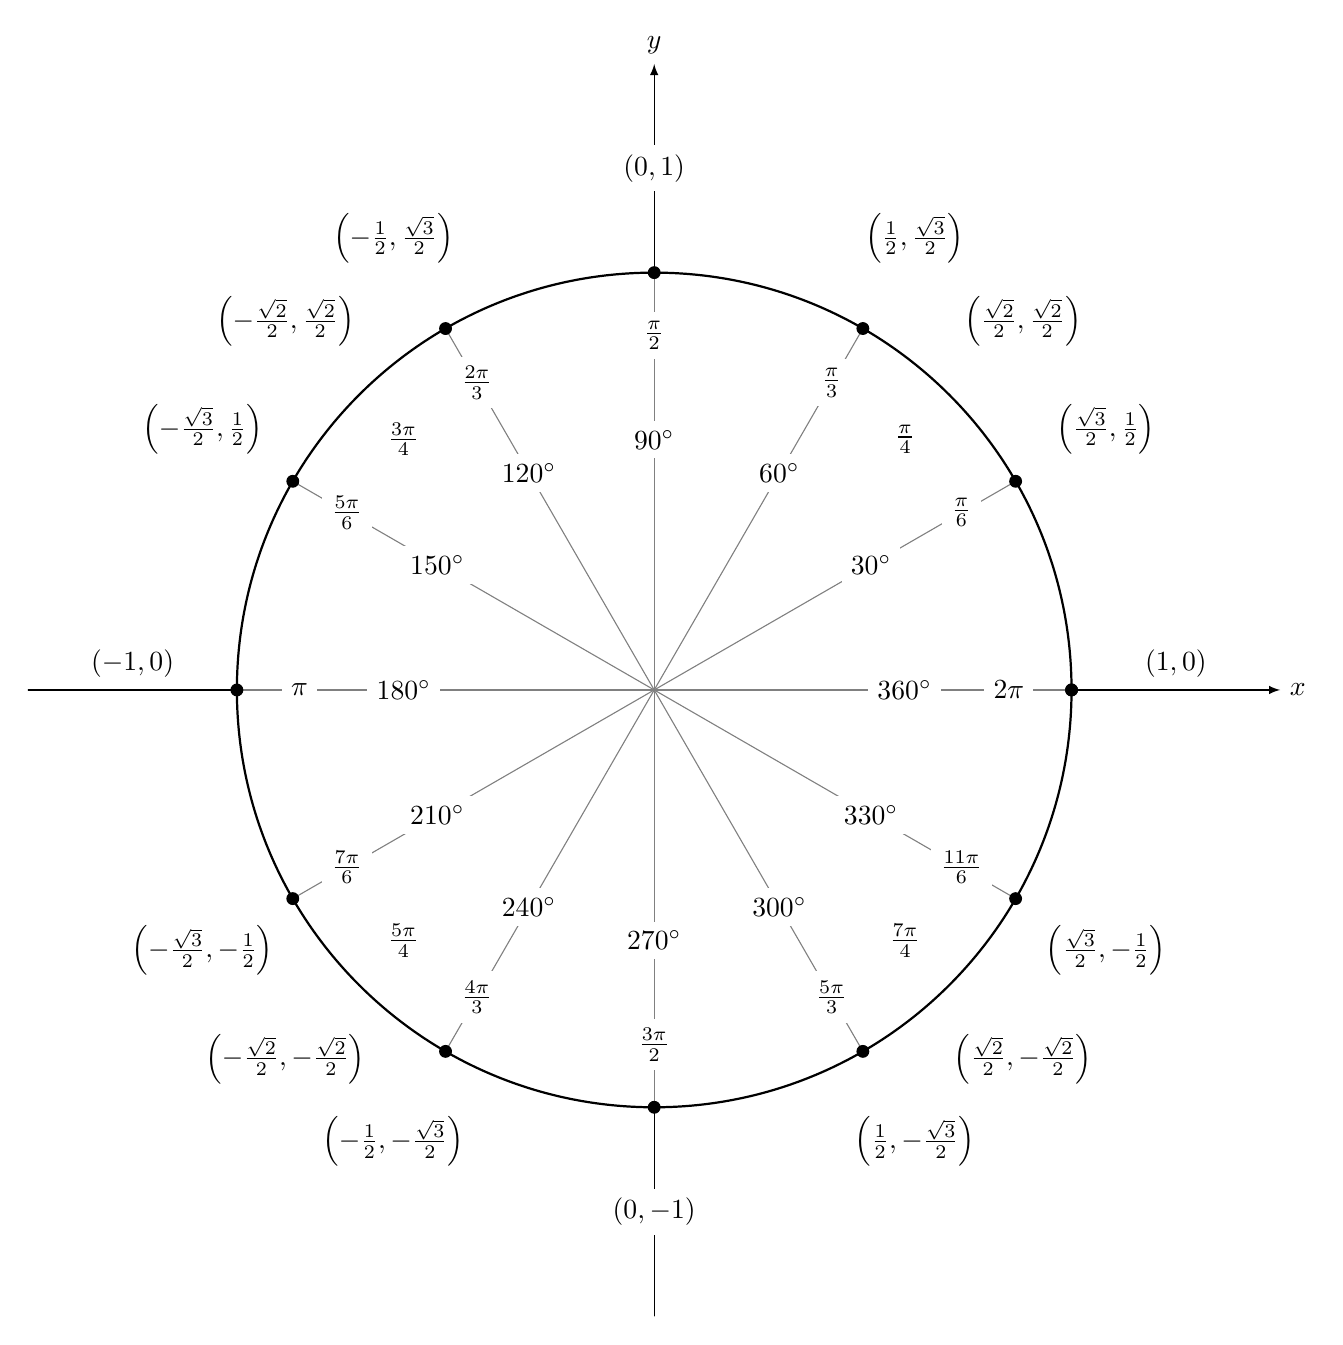
\begin{tikzpicture}[scale=5.3,cap=round,>=latex]
        % draw the coordinates
        \draw[->] (-1.5cm,0cm) -- (1.5cm,0cm) node[right,fill=white] {$x$};
        \draw[->] (0cm,-1.5cm) -- (0cm,1.5cm) node[above,fill=white] {$y$};

        % draw the unit circle
        \draw[thick] (0cm,0cm) circle(1cm);

        \foreach \x in {0,30,...,360} {
                % lines from center to point
                \draw[gray] (0cm,0cm) -- (\x:1cm);
                % dots at each point
                \filldraw[black] (\x:1cm) circle(0.4pt);
                % draw each angle in degrees
                \draw (\x:0.6cm) node[fill=white] {$\x^\circ$};
        }

        % draw each angle in radians
        \foreach \x/\xtext in {
            30/\frac{\pi}{6},
            45/\frac{\pi}{4},
            60/\frac{\pi}{3},
            90/\frac{\pi}{2},
            120/\frac{2\pi}{3},
            135/\frac{3\pi}{4},
            150/\frac{5\pi}{6},
            180/\pi,
            210/\frac{7\pi}{6},
            225/\frac{5\pi}{4},
            240/\frac{4\pi}{3},
            270/\frac{3\pi}{2},
            300/\frac{5\pi}{3},
            315/\frac{7\pi}{4},
            330/\frac{11\pi}{6},
            360/2\pi}
                \draw (\x:0.85cm) node[fill=white] {$\xtext$};

        \foreach \x/\xtext/\y in {
            % the coordinates for the first quadrant
            30/\frac{\sqrt{3}}{2}/\frac{1}{2},
            45/\frac{\sqrt{2}}{2}/\frac{\sqrt{2}}{2},
            60/\frac{1}{2}/\frac{\sqrt{3}}{2},
            % the coordinates for the second quadrant
            150/-\frac{\sqrt{3}}{2}/\frac{1}{2},
            135/-\frac{\sqrt{2}}{2}/\frac{\sqrt{2}}{2},
            120/-\frac{1}{2}/\frac{\sqrt{3}}{2},
            % the coordinates for the third quadrant
            210/-\frac{\sqrt{3}}{2}/-\frac{1}{2},
            225/-\frac{\sqrt{2}}{2}/-\frac{\sqrt{2}}{2},
            240/-\frac{1}{2}/-\frac{\sqrt{3}}{2},
            % the coordinates for the fourth quadrant
            330/\frac{\sqrt{3}}{2}/-\frac{1}{2},
            315/\frac{\sqrt{2}}{2}/-\frac{\sqrt{2}}{2},
            300/\frac{1}{2}/-\frac{\sqrt{3}}{2}}
                \draw (\x:1.25cm) node[fill=white] {$\left(\xtext,\y\right)$};

        % draw the horizontal and vertical coordinates
        % the placement is better this way
        \draw (-1.25cm,0cm) node[above=1pt] {$(-1,0)$}
              (1.25cm,0cm)  node[above=1pt] {$(1,0)$}
              (0cm,-1.25cm) node[fill=white] {$(0,-1)$}
              (0cm,1.25cm)  node[fill=white] {$(0,1)$};
    \end{tikzpicture}
    $x=\cos{\theta},\quad y=\sin{\theta}$
\subsection{Algebraiske egenskaber}
\begin{enumerate}
    \item \textbf{Kommutative lov} -- $z_1+z_2=z_2+z_1$ og $z_1z_2=z_2z_1$
    \item \textbf{Associative lov} -- $(z_1+z_2)+z_3=z_1+(z_2+z_3)$, osv.
    \item \textbf{Distributive lov} -- $z_1(z_2+z_3)=z_1z_2+z_1z_3$
    \item \textbf{Nul- og enhedselement} -- $z_1+0=z_1$ og $z_1\cdot1=z_1$
    \item \textbf{Modsatte tal} -- for hvert komplekst tal $z$, findes der et komplekst tal $-z$ hvor $z+(-z)=0$
    \item \textbf{Inverse tal} -- for hvert komplekst tal $z\neq0$, findes der et komplekst tal $w$ hvor $zw=1$
\end{enumerate}
\subsection{Trekantsuligheden}
Ved komplekse tal $z$ og $w$ vil der gælde at \begin{equation}
    |x+w|\leq|z|+|w|
\end{equation}
\section{Den Komplekse Eksponentialfunktion}\label{eks}
Et komplekst tal $z=a+ib$ kan udtrykkes\begin{equation}
    e^z=e^a(\cos{b}+i\sin{b})
\end{equation}hvor $e^z$ er et komplekst tal med modulus $e^a$ og argumentet $b$. Der gælder desuden at $z=re^{i\theta}$.
\section{$n$-te rødder}
\begin{theorem}{$n$-te rødder af et komplekst tal.}
$z\in\mathbb{C}$, hvor at $w\in\mathbb{C}$ er en $n$-te rod af $z$ hvis $w^n=z$. Alle disse rødder kan findes således, når $z=re^{i\theta}$. Da har vi\begin{align}
    w_0&=r^{\frac{1}{n}}e^{i\frac{\theta}{n}}\\
    w_1&=r^{\frac{1}{n}}e^{i\left(\frac{\theta}{n}+\frac{2\pi}{n}\right)}\\
    &\ldots\\
    w_{n-1}&=r^{\frac{1}{n}}e^{i\left(\frac{\theta}{n}+\frac{2\pi(n-1)}{n}\right)}
\end{align}
Så vil der altså gælde at $z=re^{i\theta}$ præcist har $n$ $n$-rødder givet ovenover.
\end{theorem}
\section{Komplekse 2.gradsligninger}
Vi har en ligning \begin{equation}
    az^2+bz+c=0,\,\quad\text{ hvor }a\neq0
\end{equation}Rødderne er givet ved \begin{equation}
    \frac{-b\pm i\sqrt{4ac-b^2}}{2a}
\end{equation}
Rødder vil blot være hinandens konjugerede.
\subsection{Algebraens fundamentalsætning}
Hvis $p(z)=c_hz^n+\ldots+c_1z+c_0,c_n\neq0$, da findes $r_1,\ldots,r_n\in\mathbb{C}$ så $p(n)=c_n(z-r_1)(z-r_2)\cdots(z-r_n)$.

Se desuden på et polynomium $P(x)$ og et tal $\alpha$. Vi kan dividere disse, og få en kvotient og rest:$$P(x)=(x-\alpha)\cdot Q(x)+r$$hvor der gælder at $\alpha$ er rod i $P(x)$ $\iff$ $r=0$.